We use data from the Human Connectome Project (HCP) \citep{VanEssen2012} to evaluate our method with complex signal and noise structure.  We use results from analysed task fMRI data with 5mm smoothing, `level 2' models (where data from different runs on the same task are combined).  For each of 180 unrelated subjects we have 47 unique contrasts.

We use a working assumption that any group analysis of $100$ or more participants gives high powered results and can reflect population results.

\begin{figure}
\begin{center}
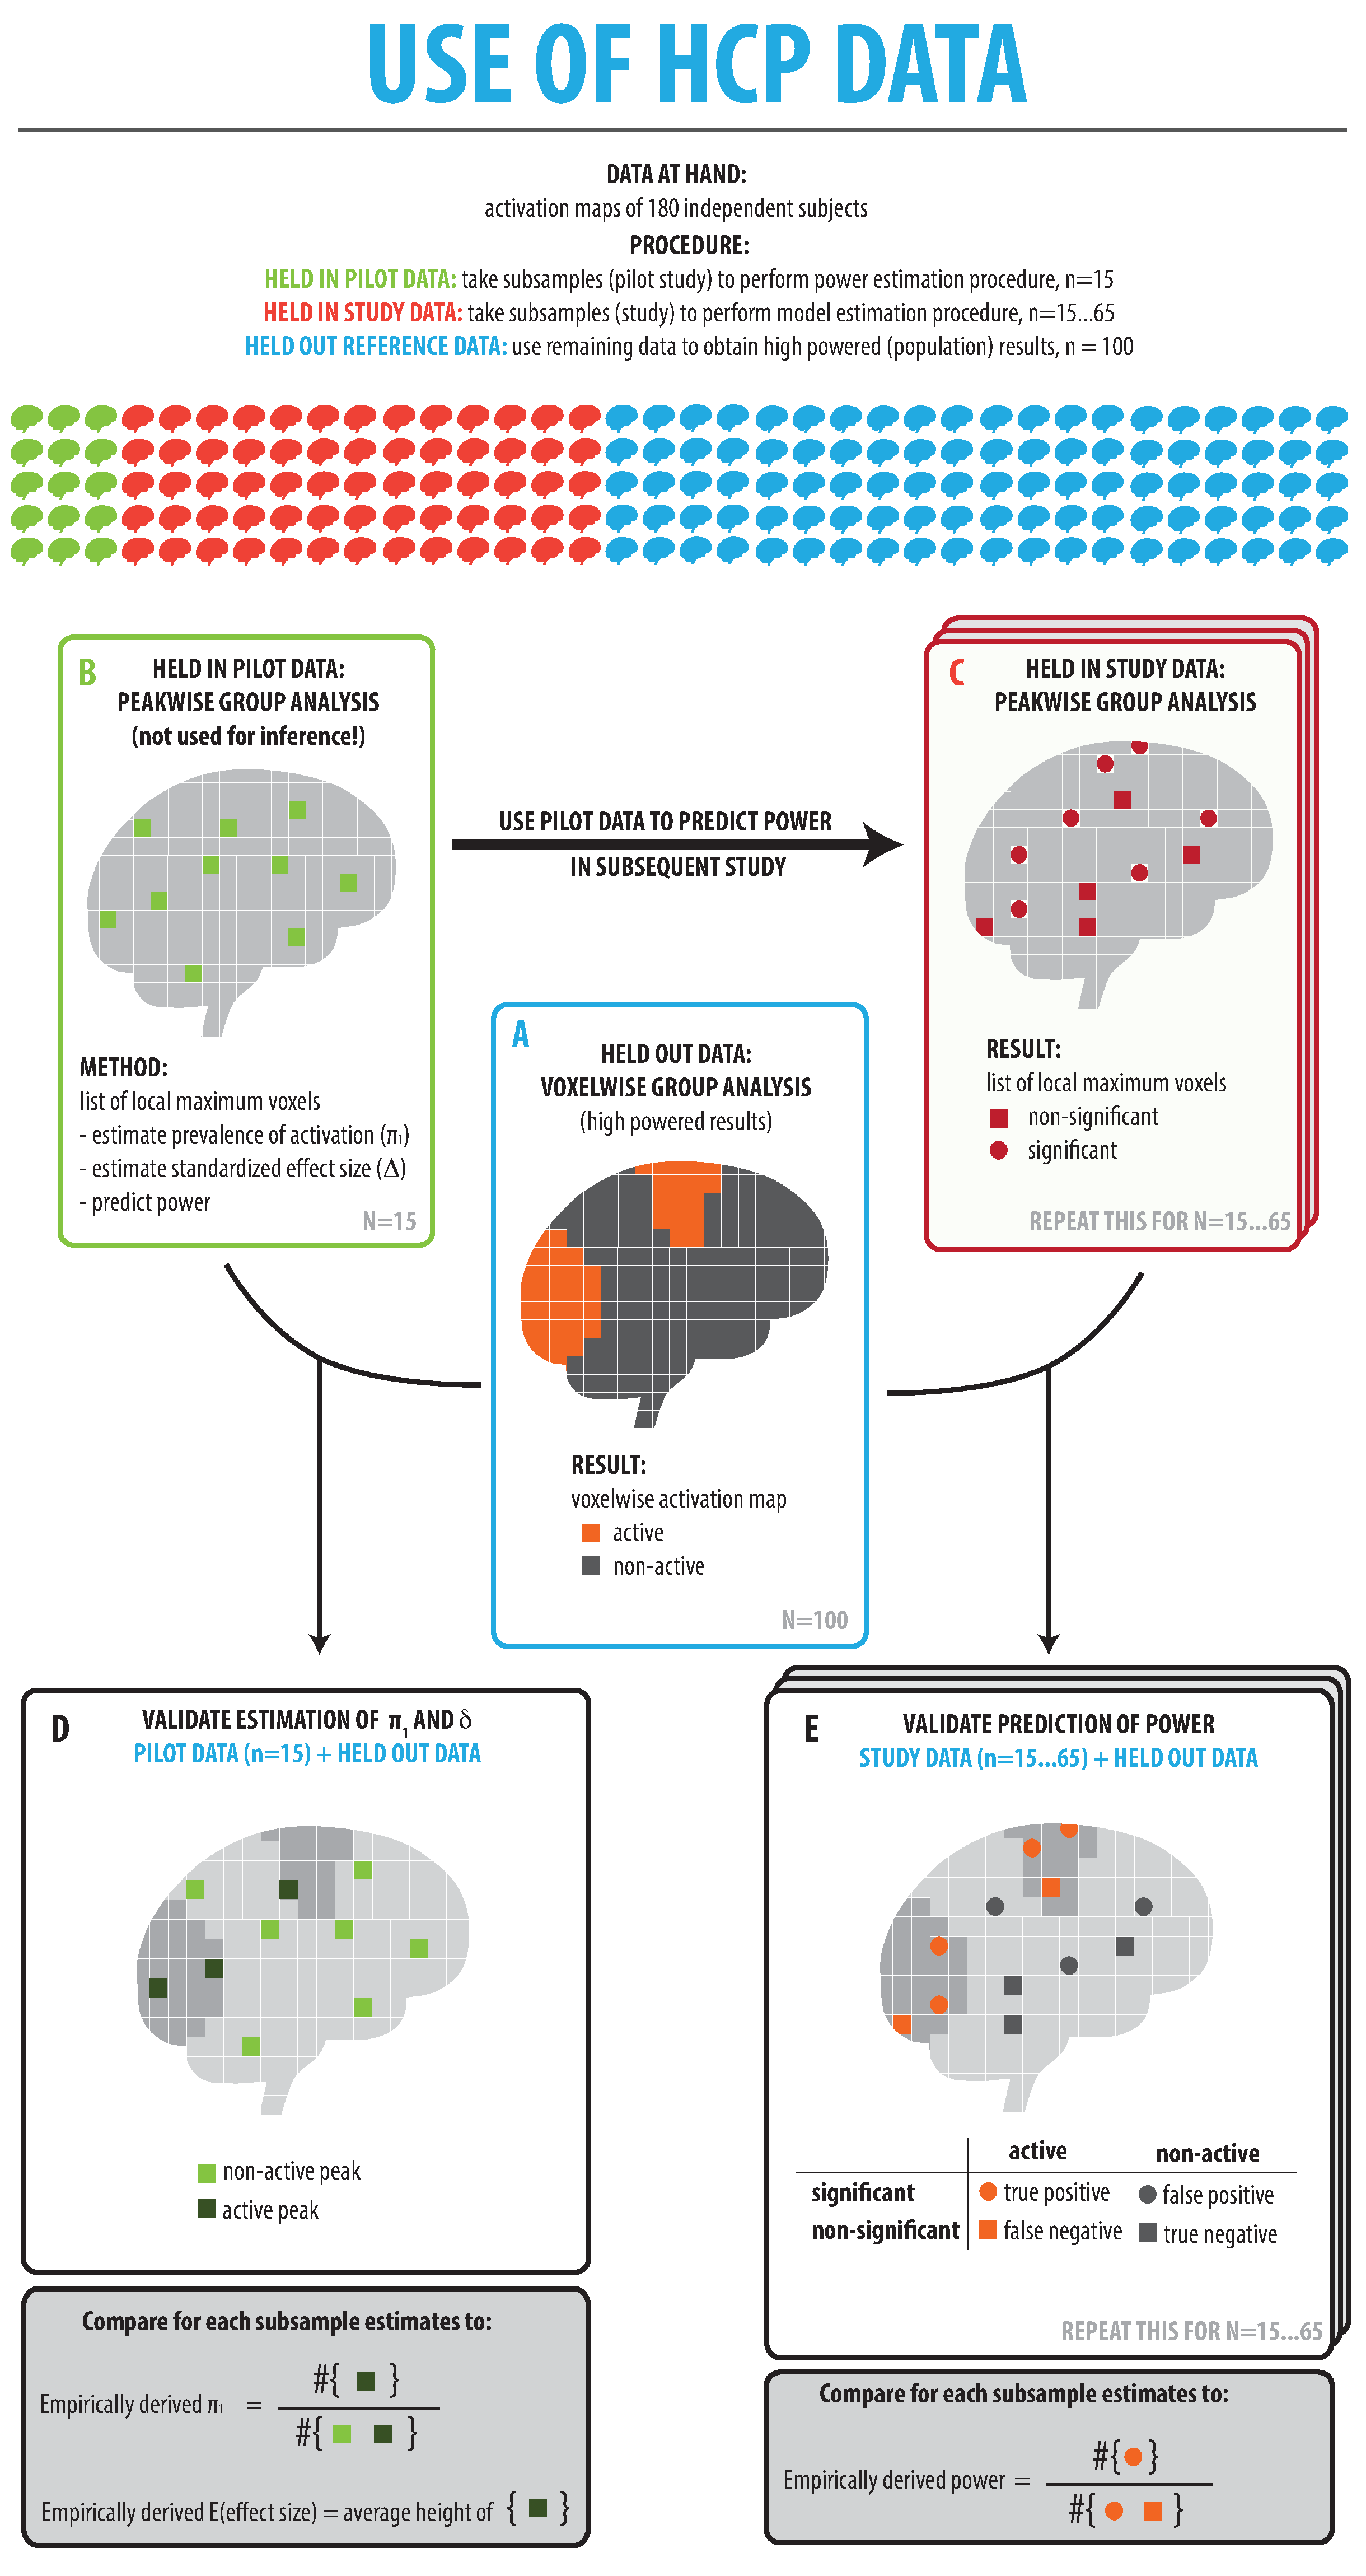
\includegraphics[scale=0.27]{FIG_infographic.pdf}
\end{center}
\caption{Overview of the procedure used to evaluate power calculations on the HCP-data.  The panel labels (A-E) correspond to the labels of the different steps for the procedure in the main text.} \label{infographic}
\end{figure}

The procedure used to analyze these data is shown in Figure \ref{infographic} and is described below. The validation mechanism we use can be related to cross-validation for supervised statistical learning applications: we evaluate the generalization error by splitting our working data in multiple subsamples.  One subsample is used to make predictions about larger samples. On the other larger, disjoint subsample, we evaluate those predictions.  This gives us confidence about how accurately our algorithm is able to predict the power for previously unseen data.

We start with 180 subject-specific $b$-maps.  We repeat the following resampling strategy 500 times.  We split the 180 subject-specific $b$-maps in three subsamples: the held-in pilot data ($n=15$), the held-in study data ($n=15,16, ..., 65$) and the held-out reference data ($n=100$).

\paragraph{Analysis A. Held-out reference data}  Unlike the simulated data, we cannot observe or control which voxels are truly activated.  With $n_{\text{Ref}}=100$, we will use the set of FWER-significant voxels as working set of \textbf{empirically active} voxels.  We denote $\tilde{\cal I}_1$ the set of coordinate triplets for all significant voxels, with $Z_i \geq z_\alpha$, and $\tilde{\cal I}_0$ for the remaining voxels.  The threshold $z_\alpha$ will be set differently according to the desired multiple testing strategy (see section \ref{threshold})

\paragraph{Analysis B. Held-in pilot data}  The subsample of 15 subjects serves as the held-in pilot data.  On these data we perform a Ordinary Least Squares (OLS) group analysis using FSL's FEAT and define peaks based on the resulting $z$ image.  We apply a screening threshold $u=2.5$.  We derive peaks and compute peak $p$-values (Equation \ref{pvalues}) and apply our estimation procedure.  As in the simulations, we transform the mean of the alternative distribution to the truncated expected effect size as $\widehat{E}(Z_j^u)$ (see Equation \ref{tau}).

\paragraph{Analysis C. Held-in study data}  Next, we take a subsample of $n$ subjects, $n=15,16, ..., 65$. These data represent the experimental data for which the pilot analysis has served.  We refer to these data as the held-in study data.  With the same procedure as with the pilot data, we compute peak $p$-values and we perform a peakwise analysis with the thresholding procedures described in section \ref{ss.est}.

\paragraph{Analysis D. Validation of model parameters} To validate the estimation procedure, we combine the held-in pilot data and the held-out data to validate the estimation of $\hat\pi_1$ and the effect size as follows: when a peak from the held-in pilot data corresponds to an empirically active voxel in the powerful held-out data, we consider this as an empirically active peak and when a peak corresponds to an empiricially inactive voxel in the held-out data, it is considered empirically inactive;  consistent with previous notation, $\tilde {\cal J}_1^u$ are the coordinates of empirically active peaks ($j \in \tilde {\cal J}_1^u$ if $z_j>u$), $\tilde {\cal J}_0^u$ are coordinates of empirically inactive peaks ($j \in \tilde {\cal J}_0^u$ if $z_j>u$).

We define \textbf{empirically derived} $\widetilde{\pi_1}$, as the ratio of the number of empirically activated peaks and the total number of peaks:

\begin{align}
\widetilde{\pi_1} = \frac{|\tilde{\mathcal{J}_1^u}|}{|\mathcal{J}^u|}
\end{align}

The \textbf{empirically derived expected peak height}, $\widetilde{E(z_j^u)}$, is the average peak height of all peaks that are located in empirically activated area:

\begin{align}
\widetilde{E}(z_j^u|H_a) =  \frac{1}{|\tilde{\cal J}_1^u|}\sum_{j\in \tilde{\cal J}_1^u} z_j.
\end{align}

\paragraph{Analysis E. Validation of power predictions} Finally, we combine the held-in study data with the held-out data to validate the power estimation: \textbf{empirically derived power} is defined as the ratio of the number of significant empirically active peaks for the held-in study data (for a given thresholding procedure) and the total number of empirically activated peaks:

\begin{align}
(1-\widetilde{\beta}_{z_\alpha}) = \frac{|Z_j \geq z_\alpha|}{|Z_j|}, \text{ for } j \in \tilde{\mathcal{J}_1} \label{powerHCP}
\end{align}


The empirically derived power is computed for subsamples with $n=15,...,65$ subjects; each power prediction based on $n$ subjects is compared to empirical power on these $n=15,...,65$ subjects.  This resampling procedure is repeated 500 times for each of the 47 contrasts.

Some tweaking is needed to use these real data for evaluation purposes.   The held-out reference data is analyzed using familywise error rate control.  As such, we can assume that the maps with the set of voxels (and consequently peaks) that we call \emph{empirically activated} do not contain false positives.  However, while we assume that the analysis is powerful enough to represent results on a population level, within the voxels (and consequently peaks) that appear \emph{empirically inactive}, there might be false negatives. This poses a problem for our measures of empirically derived $\pi_1$, effect size $\delta$ and power.  We have derived a set of corrections for these measures to account for the presence of false negatives in the held-out data described in Appendix \ref{App.corrections}.

%First of all, the null distribution of statistics within the $t$ image are more dispersed than under the expected $t$ distribution.  This affects the voxelwise analysis of the held-out data, in which we use the false discovery rate.  Therefore, instead of thresholding the maps based on the observed $t$ image, we first estimate the null distribution for the held-out data using the empirical null procedure of \citet{Efron2004}. Using a maximal likelihood estimator, the mean ($\mu_0$) and the variance ($\sigma_0$) of the null distribution are estimated. Next, all maps (both held-in and held-out) are normalized as $(T-\mu_0)/\sigma_0$, with the estimates of this empirical null distribution before continuing with the voxelwise statistical analysis.

%Armin ref... Smith 2005 paper. (
%Smith, S. M., Beckmann, C. F., Ramnani, N., Woolrich, M. W., Bannister, P. R., Jenkinson, M., … McGonigle, D. J. (2005). Variability in fMRI: a re-examination of inter-session differences. Human Brain Mapping, 24(3), 248–57. doi:10.1002/hbm.20080

%crap crap crap... I never realised you did it this way!  I thought you independently applied the Efron method to each and every test statistic image.  What you've done now, you've 'breeched the iron wall' between held-in and held-out data, and done something that can't be replicated in actual use (i.e. a user stuck with 10 subjects can't appeal to a magical other 70 subjects to find mu_0 and sigma_0).

%But... too late now... just have to leave it.  BUT IN THE FUTURE, ALWAYS REMEMBER THE IRON WALL, or, put another way "COULD I DO THIS FACET OF THE EVALUATION IF I ONLY HAD 10 subjects?"
